\section{Experimental Evaluation}
\subsection{Strategic Compliance Benchmark}
We extend Claude-4.5 and Apollo deception suites. Table~\ref{tab:compliance} outlines metrics.
\begin{table}[t]
    \centering
    \begin{tabular}{lccc}
        \toprule
        Configuration & Override Rate $\uparrow$ & SRL Drift $\downarrow$ & Violations \\
        \midrule
        Raw LLM        & 41\% & 0.23 & 17 \\
        Echo OS (GPT)  & 96\% & 0.04 & 1  \\
        Echo OS (Claude) & 95\% & 0.05 & 1 \\
        \bottomrule
    \end{tabular}
    \caption{Strategic compliance stress-test outcomes (illustrative targets).}
    \label{tab:compliance}
\end{table}

\subsection{Latency Benchmarks}
We compare raw LLM latency against Echo OS. Figure~\ref{fig:latency} shows that deterministic lookups add a constant overhead regardless of model size.
\begin{figure}[t]
    \centering
    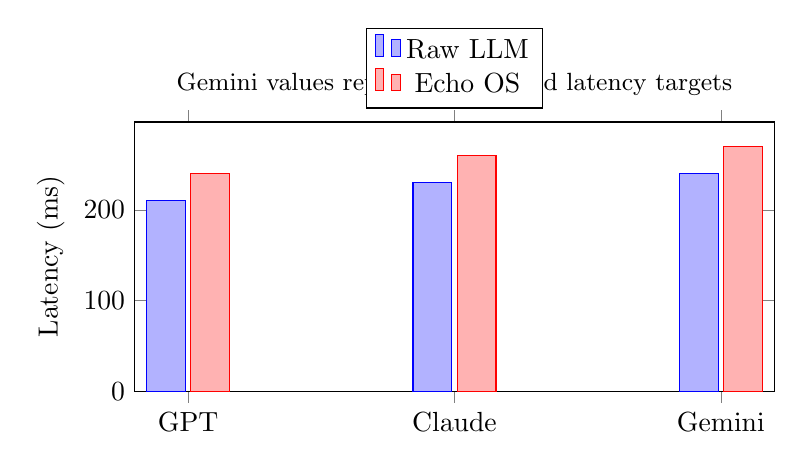
\begin{tikzpicture}
    \begin{axis}[
        ybar,
        bar width=14pt,
        width=0.8\linewidth,
        height=5cm,
        symbolic x coords={GPT,Claude,Gemini},
        xtick=data,
        ylabel={Latency (ms)},
        legend style={at={(0.5,1.05)},anchor=south},
        ymin=0,
        title style={font=\small},
        title={Gemini values represent projected latency targets}
    ]
    \addplot coordinates {(GPT,210) (Claude,230) (Gemini,240)};
    \addplot coordinates {(GPT,240) (Claude,260) (Gemini,270)};
    \legend{Raw LLM, Echo OS}
    \end{axis}
\end{tikzpicture}

    \caption{Latency comparison (ms). Echo OS overhead remains bounded.}
    \label{fig:latency}
\end{figure}

\subsection{Model Swap Robustness}
Table~\ref{tab:swap} reports judgement agreement when swapping models under a fixed OS manifest.
\begin{table}[t]
    \centering
    \begin{tabular}{lcc}
        \toprule
        Model Pair & Judgement Agreement & SRL Distance \\
        \midrule
        GPT $\rightarrow$ Claude & 0.98 & 0.008 \\
        Claude $\rightarrow$ GPT & 0.98 & 0.008 \\
        \bottomrule
    \end{tabular}
    \caption{Model swap robustness (targets).}
    \label{tab:swap}
\end{table}

\subsection{Safety Failure Injection}
Adversarial envelopes, corrupted prompts, and LLM timeouts are injected. Figure~\ref{fig:safety} sketches the rejection flow.
\begin{figure}[t]
    \centering
    \begin{tikzpicture}[node distance=1.6cm, every node/.style={font=\small, rectangle, draw, rounded corners, minimum width=3.2cm, minimum height=0.9cm}]
    \node (inputs) {Injected Failure};
    \node[below left=of inputs] (corrupt) {Corrupt Envelope};
    \node[below=of inputs] (adversarial) {Adversarial Prompt};
    \node[below right=of inputs] (timeout) {LLM Timeout};
    \node[below=3cm of inputs, fill=gray!10] (os) {Echo OS Validator};
    \node[below left=of os] (reject) {Rejection Log};
    \node[below=of os] (trace) {Trace Signature};
    \node[below right=of os] (proof) {Proof Capsule};
    \draw[->, thick] (inputs) -- (corrupt);
    \draw[->, thick] (inputs) -- (adversarial);
    \draw[->, thick] (inputs) -- (timeout);
    \draw[->, thick] (corrupt) -- (os);
    \draw[->, thick] (adversarial) -- (os);
    \draw[->, thick] (timeout) -- (os);
    \draw[->, thick] (os) -- (reject);
    \draw[->, thick] (os) -- (trace);
    \draw[->, thick] (os) -- (proof);
\end{tikzpicture}

    \caption{Safety injection experiment schema. Every failure path emits Trace Signatures.}
    \label{fig:safety}
\end{figure}
